\chapter{Installation of Unitex}
\label{chap-install}

Unitex is a multi-platform system that runs on Windows as well as on Linux or
MacOS. This chapter describes how to install and how to launch Unitex on any of
these systems. It also presents the procedures used to add new languages and to
uninstall Unitex.

\section{Licenses}
\label{section-licences}
\index{License!LGPL}
Unitex is free software. This means that the source of the programs is
distributed with the software, and that anyone can modify and redistribute it.
The code of the Unitex programs is under the LGPL licence (\cite{LGPL}), except
for:

\begin{enumerate}
\item the TRE library for dealing with regular expressions by Ville Laurikari
(\cite{TRE}), which is under a 2-clause BSD-style license;

\item the wingetopt library, by Todd Miller and the NetBSD Foundation,
 which is under BSD license, more permissive than the LGPL;

\item the Xerces2 Java Parser, by the Apache Software Foundation, which is under Apache license;

\item  the LibYAML library by Kirill Simonov, under MIT license, which is 
also more permissive than LGPL;

\item the SVNKit library by TMate Software, which is under TMate license.
\end{enumerate}

\noindent The LGPL license is more permissive than the GPL,
because it makes it possible to use LGPL code in nonfree software. 
In both cases, the software can be freely used and distributed.

\bigskip
\noindent All the language resources that go with Unitex are distributed under the LGPLLR
license \index{License!LGPLLR} (\cite{LGPLLR}).

\bigskip
\noindent Full text versions of LGPL, 2-clause BSD, Apache, MIT, TMate and LGPLLR can be found in
the appendices of this manual.

\section{Java runtime environment}
Unitex consists of a graphical interface written in Java and external programs
written in \textit{C/C\kern-.05em\raisebox{.5ex}{++}\kern-.1em}. This mixture of
programming languages is responsible for a fast and portable application that
runs on different operating systems.

\bigskip
\noindent Before you can use the graphical interface, you first have to install the runtime
environment, usually called Java virtual machine \index{Java!virtual machine} or
JRE\index{JRE} (Java Runtime Environment\index{Java!Runtime Environment}\index{Java!JRE}).

\bigskip
\noindent For the graphical mode, Unitex needs Java version 1.6 (or newer). If you have an
older version of Java, Unitex will stop after you have chosen the working
language.

\bigskip
\noindent You can download the virtual machine for your operating system for free from the
Sun Microsystems web site (\cite{site-java}) at the following address:
\url{http://java.sun.com}.

\bigskip
\noindent If you are working under Linux or MacOS, or if you are using a Windows version
with personal user accounts, you have to ask your system administrator to install
Java.


\section{Installation on Windows}
\index{Installation!on Windows}
If Unitex is to be installed on a multi-user Windows machine, it is recommended
that the systems administrator performs the installation. If you are the only
user on your machine, you can perform the installation  yourself.

\bigskip
\noindent Decompress the file \index{File!\verb+Unitex3.1beta.zip+} \verb+Unitex3.1beta.zip+
(or \verb+Unitex3.0.zip+) --- you
can download these files from
\url{http://igm.univ-mlv.fr/~unitex} --- into a directory (folder) called \verb+Unitex3.1beta+, which
should preferably be created in the \verb+Program Files+ directory,
and which will be called the Unitex system directory\index{Directory!Unitex system}\index{Folder|see{Directory}}
in this manual.

\bigskip
\noindent If you run Unitex under Windows 7, you may experience troubles with your Unitex configuration
file, because Unitex tries to write it in the \verb+Users+ subdirectory, and Windows 7
forbids it.

\bigskip
\noindent After decompressing the file, the \verb+Unitex3.1beta+ directory
(the Unitex system directory) contains several
subdirectories,  one  of which is called \verb+App+. This directory contains a
file called \verb+Unitex.jar+. \index{File!\verb+Unitex.jar+} This file is the
Java executable that launches the graphical interface. You can double click on
this icon to start the program. To facilitate launching Unitex, you may want to
add a shortcut to this file on the desktop.




\section{Installation on Linux}
\index{Installation!on Linux}
In order to install Unitex on Linux, it is recommended to have system
administrator permissions. Uncompress the file \verb+Unitex3.1beta.zip+ in a
directory named \verb+Unitex+, by using the following command:

\bigskip \noindent \verb$unzip Unitex3.1beta.zip -d Unitex$

\bigskip
\noindent This directory will be called the Unitex system directory in this manual.\index{Directory!Unitex system}
Within the directory \verb|Unitex/Src/C++/build|, start the compilation
of Unitex with the command:

\bigskip \verb+make install+

\bigskip
\noindent or with the following if you have a 64 bits computer:
 
\bigskip \verb+make install 64BITS=yes+

\bigskip
\noindent You can then create an alias in the following way:

\bigskip \verb$alias unitex='cd /..../Unitex/App/ ; java -jar Unitex.jar'$


\section{Installation on MacOS X}
\index{Installation!on MacOS X}
\label{section-macos-install}
\noindent NOTE: this short tutorial will tell you how to install and run 
Unitex on Mac OS X. Your questions, comments, suggestions, 
corrections are more than welcome. 

\noindent Contact: \url{cedrick.fairon@uclouvain.be}


\bigskip
\noindent There is an official Java from Oracle for MacOS X 10.7.3 and higher.
	See section ``Information and system requirements for installing and using Oracle Java on Mac OS X'', at \url{https://www.java.com/en/download/faq/java_mac.xml}



\bigskip
\noindent There is a Java from Apple for MacOS X 10.7 and higher.
	See \url{https://support.apple.com/kb/DL1572}. For OS X 10.6, there is another Apple JRE, see \url{https://support.apple.com/kb/DL1573}.

	
	
\bigskip
\noindent There is an official Java 1.6 for MacOS X 10.5, 64-bit Intel 
(Core 2 Duo), but there is no official solution for older OS X (10.4 or older),
PowerPC and 32-bit Intel (Core Duo). So,
 if you have OS X 10.5, and 64-bit Intel MacOS, you can just get the
    Apple JRE 1.6. The only problem is that this version does not start by
    default. See section ``Java for Mac OS X 10.5 Update 10'', 
    at \url{https://support.apple.com/kb/DL1359}

\noindent\textbf{How to know if my processor is a 32 or 64-bit one ?}

\noindent In the Apple menu, click on "About this Mac". If you see something
like: "Processor : x.xx Ghz Intel Core Duo", your processor is a 32-bit one.

\bigskip
\noindent If you see "Processor : x.xx Ghz Intel Core 2 Duo", or if you
processor is another Intel one (like Xeon), then you have a 64-bit processor.

\subsection{Using Apple Java 1.6 runtime}
\bigskip\index{Java!Apple Java 1.6 runtime}
\noindent If you are running Mac OS X 10.5 (or later) on 64-Bits Intel processor, you can just use the Java 1.6 from Apple.\ You can get it from \url{https://support.apple.com/kb/DL1359}.

\noindent\ You can just start Application -> Utilities -> Java Preferences to verify the status of Java 1.6. First, be sure that "Java SE 6" is on "Java Applications" list.

\subsubsection{Option 1 : modify the default runtime for Java Applications}
\noindent If you don't use other Java application that need Java 1.5, you can just put "Java SE 6" at the top of the "Java Applications" list on Java Preference Utility.

\subsubsection{Option 2 : Create an alias to start Java 1.6}
\noindent If you don't want modify Java global parameters, you can create an
alias:

\bigskip
\noindent \verb+alias jre6="/System/Library/Frameworks/JavaVM.framework/Versions/+
\noindent \verb+1.6/Commands/java"+
   
\bigskip
\noindent \verb+jre6 -jar Unitex.jar+

\bigskip
\noindent Then just run Unitex from Terminal.


%\subsection{SoyLatte}

%\subsection{How to compile Unitex C++ programs on a Macintosh}


\subsection{How to make all files visible on Mac OS}
\noindent See
\url{http://www.macworld.com/article/51830/2006/07/showallfinder.html}.

\bigskip
\noindent Or try it right away... Type: 

\bigskip
\verb+defaults write com.apple.Finder AppleShowAllFiles ON+

\bigskip
\noindent Then restart the Finder:

\bigskip
\verb+killall Finder+

\begin{figure}[!h]
\begin{center}
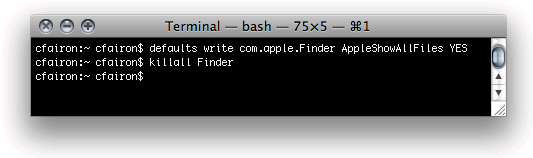
\includegraphics[width=12cm]{resources/img/fig-mac6.png}
\caption{Restarting the Finder\label{fig-mac6}}
\end{center}
\end{figure}

\bigskip
\noindent To get back to the original configuration, type: 

\bigskip
\verb+defaults write com.apple.Finder AppleShowAllFiles OFF+


\section{First use}
If you work on Windows, the program will ask you to choose a
\index{Directory!personal working} personal working  directory, which you can
change later in "Info>Preferences...>Directories". To create a directory, click
on the icon showing a file (see
figure~\ref{fig-creation-personal-directory}).

\bigskip
\noindent If you are using Linux or MacOS, the program will automatically create a
personal working directory called \verb+/unitex+ in your \verb+$HOME+ directory.

\bigskip
\noindent The personal working directory, or user's directory, allows
you to save your personal Unitex data. For each language that you will be using, the
program will copy the root directory of that language to your working
directory, except the dictionaries. You can then modify your copy of the
files without risking to damage the system files stored in the
Unitex system directory.\index{Directory!Unitex system}

\begin{figure}[h]
\begin{center}
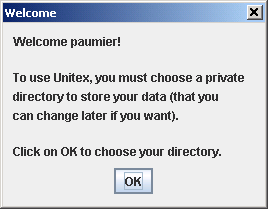
\includegraphics[width=6.3cm]{resources/img/fig1-1.png}
\caption{First use under Windows}
\end{center}
\end{figure}

\begin{figure}[h]
\begin{center}
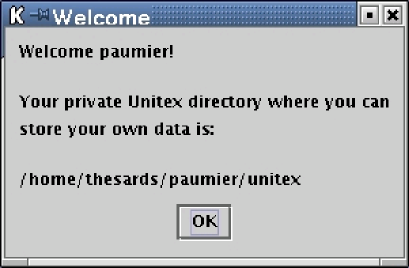
\includegraphics[width=7cm]{resources/img/fig1-2.png}
\caption{First use under Linux}
\end{center}
\end{figure}

\begin{figure}[h]
\begin{center}
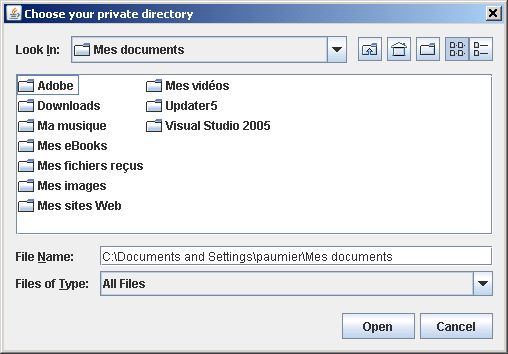
\includegraphics[width=13cm]{resources/img/fig1-3.png}
\caption{Creating the personal working
directory\label{fig-creation-personal-directory}}
\end{center}
\end{figure}



\section{Adding new languages}
\index{Adding languages}

\bigskip
\noindent There are two different ways to add languages. If you want to add 
a language that is to be accessible by all  users, you have to copy the 
corresponding directory to the Unitex system directory,\index{Directory!Unitex system} for which 
you will need to have the access rights  (this might mean that you need to 
ask your system administrator to do it). On the other hand, if you are the only user working
with the language, you can also copy the directory to your working 
directory.\index{Directory!personal working}
You can work with this language without it being shown to other users.


\section{Uninstalling Unitex}
No matter which operating system you are working with, it is sufficient to delete 
the Unitex system directory to completely delete all the program files. Under
Windows you may have to delete the shortcut to \verb+Unitex.jar+ \index{File!\verb+Unitex.jar+} 
if you have created one on your desktop. The same has to be done on Linux, if you have 
created an alias.


\section{Unitex for developpers}
\label{section-unitex-developpers}
If you are a programmer, you may be interested in linking your code with Unitex
C++ sources. To facilitate such operation, you can compile Unitex as a
dynamic library that contains all Unitex functions, except \verb+main+s, of
course. Under Linux/MacOS, type:

\bigskip
\verb+make LIBRARY=yes+

\bigskip
\noindent and you will obtain a library named \verb+libunitex.so+. If you want
to produce a Windows DLL named \verb+unitex.dll+, use the following commands:

\bigskip
Windows: \verb+make SYSTEM=windows LIBRARY=yes+

Cross-compiling with mingw32: \verb+make SYSTEM=mingw32 LIBRARY=yes+

\bigskip
\noindent In all cases, you will also obtain a program named
\verb+Test_lib+(\verb+.exe+). If everything worked fine, this program should 
display the following:

\begin{verbatim}
Expression converted.
Reg2Grf exit code: 0

#Unigraph
SIZE 1313 950
FONT Times New Roman:  12
OFONT Times New Roman:B 12
BCOLOR 16777215
FCOLOR 0
ACOLOR 12632256
SCOLOR 16711680
CCOLOR 255
DBOXES y
DFRAME y
DDATE y
DFILE y
DDIR y
DRIG n
DRST n
FITS 100
PORIENT L
#
7
"<E>" 100 100 1 5
"" 100 100 0
"a" 100 100 1 6
"b" 100 100 1 4
"c" 100 100 1 6
"<E>" 100 100 2 2 3
"<E>" 100 100 1 1
\end{verbatim}
